\chapter{相关概念及研究}
\label{ch2}

本章首先介绍了 CAV 的网络系统架构,主要从六个方面介绍,包括 TSP 云
服务、V2X 车载通信、车载网络、CAN 总线、IVI、T-BOX,分别分析了它们的
系统架构的组成和原理,最后从云平台、APP、T-BOX、IVI、CAN 总线、ECU、
车间通信七个方面介绍了智能网联汽车所面临的安全威胁

\section{智能网联汽车联网系统架构}

\subsection{车载网络架构划分}
智能网联汽车是指车联网与智能车的有机联合,是搭载先进的车载传感器、控制器、执行器等装置,并融合现代通信与网络技术,
实现车与人、路、后台等智能信息交换共享,实现安全、舒适、节能、高效行驶,并最终可替代人来操作的新一代汽车\cite{icvsintro}。
车联网在智能辅助驾驶、智能交通规划等领域,都具有不错的应用前景。
车载网络架构如图2.1所示。这是一个
以域为中心的体系结构,具有以太网作为主干,分为五个领域:动力系统、底盘、车
身、信息娱乐和高级驾驶辅助系统(ADAS)。每个域控制
器通过一个中央网关与以太网主干连接。CAN/CAN FD 和
LIN 用作每个域中的通信协议。此外,车载网络可以通
过远程信息处理单元和接口(如 OBD、USB 和 Wi-Fi)连接
到外部网络。这种集中式架构通过域控制器和以太网提
供智能网联汽车所需的计算和通信能力。然而,车辆的外部接
口也增加了。这些开放的接口给智能网联汽车带来了新的攻击
面和安全隐患。为了更好地描述安全威胁,我们提出了
基于这种架构的三层车载网络模型。
\begin{itemize}
    \item 终端节点层: 这一层包含车辆中各个域的 ECU 节点、
    传感器和执行器。这是模型的中心部分。如果受到攻
    击,它会直接影响车辆的安全。
    \item 网络通信层:该层由各种车载网络通信协议组成,如
    以太网、CAN/CAN FD、LIN 等。这一层的主要目的是传
    输数据并与之交互。
    \item 接口设备层:这一层包括各种可以与外部环境交互的通
    信设备接口,如 OBD、USB 等。
\end{itemize}
\begin{figure}
  \centering
  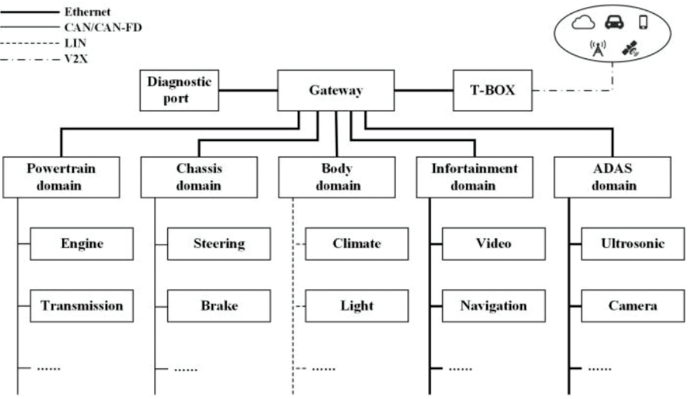
\includegraphics[scale=0.6]{resources/img/i1.png}
  \caption{车联网网络架构图}
\end{figure}
目前的汽车结构中,车辆内部网络主要由 CAN
总线和 ECU 组成。ECU 是嵌入式设备,包括各种智能系统,如无钥匙控制单元
(KCU,key control unit)、防抱死制动系统(ABS,
antilock brake system)、BCM 和紧急制动辅助
(EBA,electronic brake assist)等,通常被用于监控
车辆状态、控制车辆行为。CAN 总线是 ECU 之间
通信的桥梁,负责将汽车内部各 ECU 连接起来,
使它们能够进行高效的信息通信。
\newline
CAN 总线与大量嵌入式设备的多功能连接在为用户提供便利服务的同时,也带来了一些易入侵的接口。恶意攻击者能够利用车载信
息娱乐(IVI,in-vehicle infotainment)系统的 USB
接口和 Wi-Fi 接口恶意窃取用户隐私信息,甚至能
够利用 IVI 系统入侵 CAN 达到控制车辆的目的。
车载诊断(OBD-II,on-board diagnostics-II)接口
是美国工程师协会在 20世纪90年代制定CAN总
线规范时规定开放的车载诊断接口,通常被用来
检测汽车故障并监测汽车尾气排放。然而,OBD-II 接口也很容易成为恶意攻击者非法窃取汽车 CAN 总线数据的入口。此外,T-BOX、胎压
侦测系统(TPMS,tire pressure monitoring system)、RKE、ABS 等大量嵌入式设备都存在可被
利用的攻击面。
这里简单的介绍上述英文名词的定义。
\begin{itemize}
    \item CAN 控制器局域网(Controller Area Network,简称CAN或者CAN bus) 是一种功能丰富的车用总线标准。 
    被设计用于在不需要主机(Host)的情况下,允许网络上的单片机和仪器相互通信。 
    它基于消息传递协议,设计之初在车辆上采用复用通信线缆,以降低铜线使用量,后来也被其他行业所使用。
    \item ADAS 可帮助驾驶员进行驾驶和停车功能。通过安全的人机界面,ADAS 提高了汽车和道路的安全性。ADAS 使用传感器和摄像头等自动化技术来检测附近的障碍物或驾驶员错误,并做出相应的反应。ADAS 可以实现不同级别的自动驾驶,具体取决于车内安装的功能。
    \item OBD是英文On-Board Diagnostics的缩写,中文翻译为“车载自动诊断系统”。这个系统将从发动机的运行状况随时监控汽车是否尾气超标,一旦超标,会马上发出警示。当系统出现故障时,故障(MIL)灯或检查发动机(Check Engine)警告灯亮,
    同时动力总成控制模块(PCM)将故障信息存入存储器,通过一定的程序可以将故障码从PCM中读出。根据故障码的提示,维修人员能迅速准确地确定故障的性质和部位。
    \item ECU(Electronic Control Unit)电子控制器单元,又称为汽车的“行车电脑”,它们的用途就是控制汽车的行驶状态以及实现其各种功能。主要是利用各种传感器、总线的数据采集与交换,来判断车辆状态以及司机的意图并通过执行器来操控汽车。
    \item T-BOX作为无线网关,通过4G远程无线通讯、GPS卫星定位、加速度传感和CAN通讯等功能,为整车提供远程通讯接口,提供包括行车数据采集、行驶轨迹记录、车辆故障监控、车辆远程查询和控制(开闭锁、空调控制、车窗控制、发送机扭矩限制、发动机启停)、驾驶行为分析、4G无线热点分享等服务。
\end{itemize}
\subsection{TSP 云端通信技术}

(Telematics Service Provider)汽车远程服务提供商,在Telematics产业链居于核心地位,上接汽车、车载设备制造商、网络运营商,下接内容提供商。
 Telematics服务集合了位置服务、Gis服务和通信服务等现代计算机技术,为车主和个人提供强大的服务(导航、娱乐、资讯、安防、SNS、远程保养)。
 \begin{figure}
    \centering
    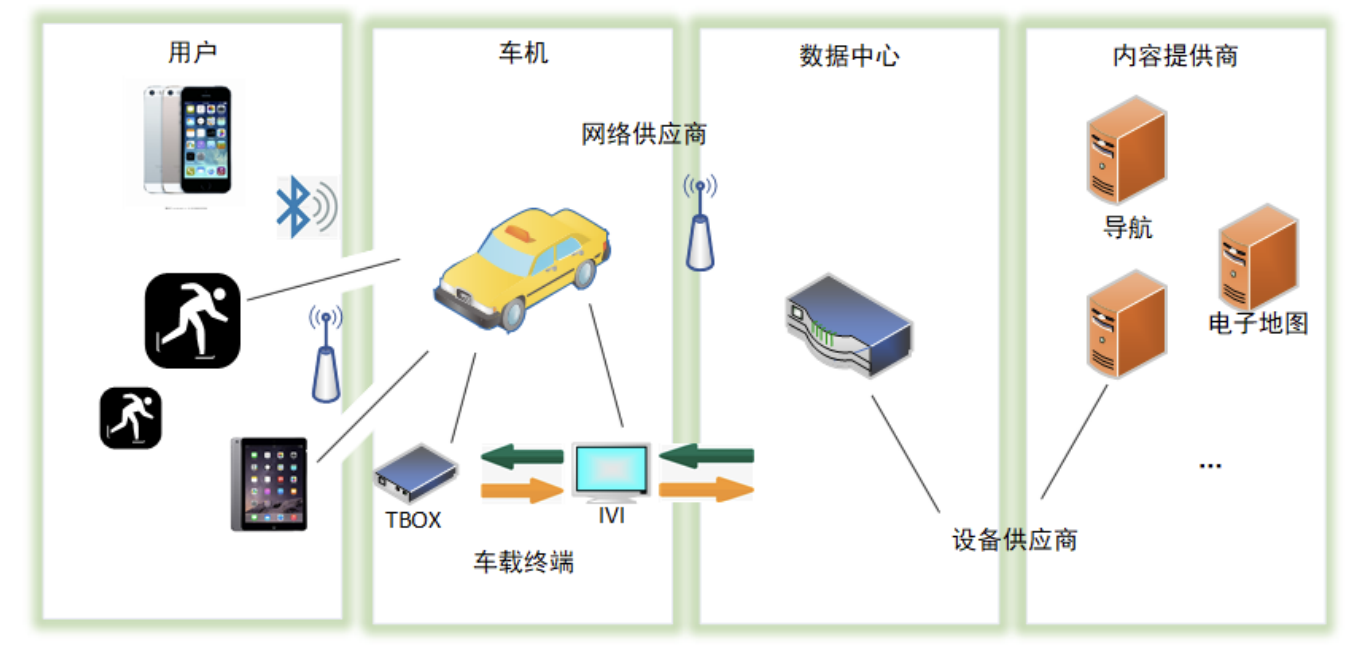
\includegraphics[scale=0.6]{resources/img/i2.png}
    \caption{TSP 系统组成}
  \end{figure}
\newline
通常所说的Telematics就是指应用无线通信技术的车载电脑系统。随着电脑和网络技术应用到汽车上,正在形成称之为Telematics的新的电脑市场。
Telematics是无线通信技术、卫星导航系统、网络通信技术和车载电脑的综合产物,被认为是未来的汽车技术之星。汽车行驶当中出现故障时,通过无线通信连接服务中心,进行远程车辆诊断,
内置在发动机上的计算机记录汽车主要部件的状态,并随时为维修人员提供准确的故障位置和原因。通过终端机接收信息并查看交通地图、路况介绍、交通信息、安全与治安服务以及娱乐信息服务等,
在后座还可以玩电子游戏、网络应用(包括金融、新闻、E-mail等)。通过Telematics提供的服务,用户不仅可以了解交通信息、临近停车场的车位状况,确认当前位置,
还可以与家中的网络服务器连接,及时了解家中的电器运转情况、安全情况以及客人来访情况。也就是说:综合上述所有功能的车载计算机系统叫Telematics。
Telematics系统运作模式就目前发展的模式观察,基本上可将其分为汽车定位系统(GPS)与资讯存取(Access)两部分。
功能特色:卫星定位、道路救援、汽车防窃、自动防撞系统、车况掌握、个人化资讯接收、多媒体娱乐资讯接收。
\newline
Telematics系统的应用领域:基本上可分为前座系统、后座系统与引擎机械系统三大子系统。前座系统主要以安全、车辆保全、驾驶简易性与舒适性为主要考量。后座系统则以多媒体娱乐为主,包括互动式游戏、高传真音响视听系统、随选视讯、数位广播与数位电视等。引擎机械系统,主要是根据车用电脑所收集的车况资讯,进行车况诊断、行车效率最佳化、远距引擎调整或零件预定等。
\newline
Telematics目前主要应用在车载系统上,根据使用目的不同,Telematics可分为三种基本类型,即交通信息与导航服务、安全驾驶与车辆保护及故障诊断的车辆维护服务、娱乐及通信服务。提供全球定位系统技术、地理信息系统、智能型交通系统技术。值得一题的是Telematics逐渐演变为综合了GPS的跟踪装置和无线通信等技术的车载系统。

TSP一词狭义的在互联汽车行业中被用作
对服务提供者进行分类的广义术语
以安全车到云为核心的汽车价值链
数据管理。然而,目前TSP扮演的传统角色
在价值链中不断进化。TSP一词已被
IT公司,系统集成商,甚至一级企业等采用。网络
运营商正在将其M2M/IOT服务扩展到
汽车行业,意图将数据连接“去商品化”。
越来越多的汽车制造商通过TSP创造和集成更多的车载部件。

\subsection{V2X 车载通信技术}

Vehicle to Everything (V2X) 是一种车载通信系统,支持将信息从车辆传输到可能影响车辆的交通系统的移动部件。V2X 技术的主要目的是提高道路安全、节能和道路交通效率。
\newline
车联网的工作原理: 在 V2X 通信系统中,信息通过高带宽、高可靠性的链路从车辆传感器和其他来源传播,使其能够与其他汽车、停车位和交通信号灯等基础设施以及使用智能手机的行人进行通信。
通过与车辆周围的其他实体共享速度等信息,该技术提高了驾驶员对潜在危险的认识,并有助于降低伤害、道路事故死亡和与其他车辆碰撞的严重程度。
该技术还通过警告驾驶员即将到来的交通、建议替代路线以避免交通和识别可用停车位来提高交通效率。
\newline
V2X 技术的组成部分:
V2X技术的关键组成部分包括V2V(车对车)和V2I(车对基础设施)。V2V 允许车辆与道路上的其他车辆进行通信,而 V2I 允许车辆与外部实体进行通信,例如交通信号灯、停车位、骑自行车的人和行人。这些技术有助于改善道路安全、减少燃料消耗并增强驾驶员与其他道路使用者(例如骑自行车者和行人)之间的体验。

当 V2X 系统集成到传统车辆中时,驾驶员可以接收有关天气模式、附近事故、道路状况、道路工程警告、紧急车辆接近以及使用同一条道路的其他驾驶员活动的重要信息。

配备 V2X 系统的自动驾驶汽车可以为车辆现有的导航系统提供更多信息。该系统还使自动驾驶汽车能够扫描周围环境并根据收到的信息立即做出决定。
\begin{figure}
    \centering
    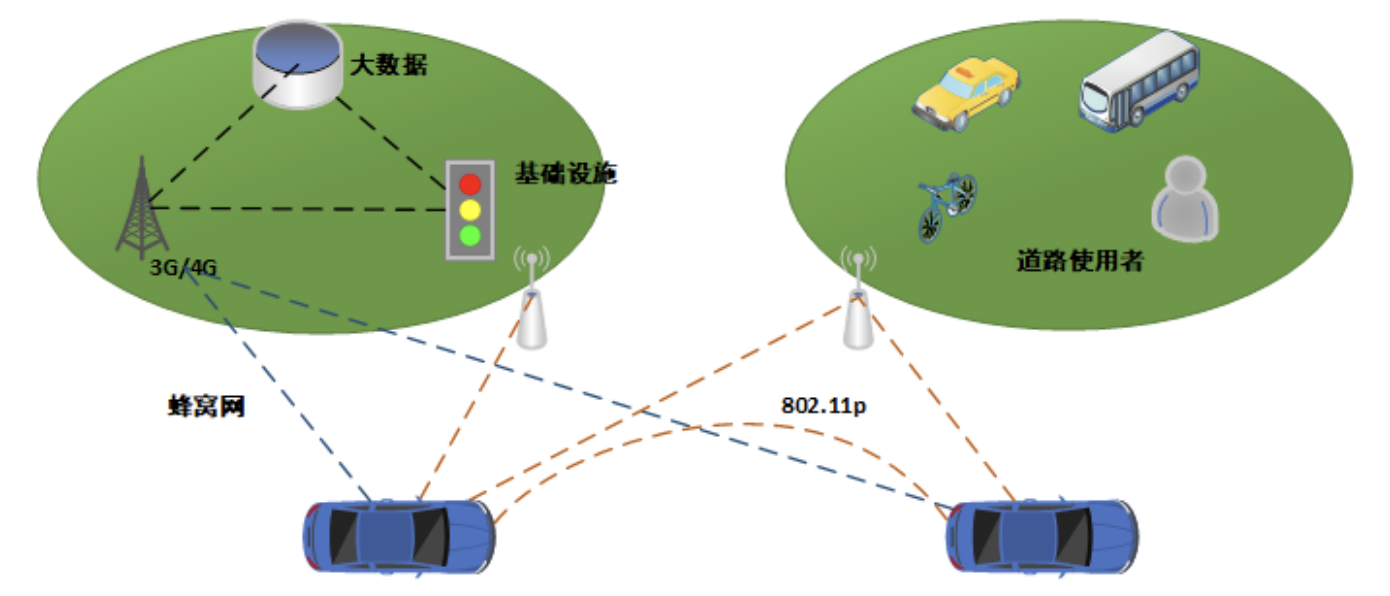
\includegraphics[scale=0.6]{resources/img/i3.png}
    \caption{v2x 应用场景}
  \end{figure}
\newline
如图2.3所示,是基于 V2X 简单的一个应用场景。智能网联汽车不仅可以借
助蜂窝网络,使得汽车与基站、云平台、路边单元等基础设备相连接实现 V2I,
而且还可以通过基站,与周围的车辆进行连接,从而实现 V2V。智能网联汽车在
与其他基础设备、非机动车、车辆、行人等进行通信的时候,使用诸如 802.11p
等协议。

\subsection{车载内部网络通信技术}
现代车载通信系统中有五种最广泛使用的车载网络:LIN(本地互连网络)、CAN(控制器局域网)、FlexRay、以太网和 MOST(面向媒体的系统传输)。各有优势和劣势。
根据实际观察,LIN 经常用于通常不需要严格时序性能的低速通信。CAN 广泛部署在动力总成和车身控制领域,也是从车辆中检索 OBD(车载诊断)数据的标准接口。
FlexRay 具有高确定性和容错性,
这通常在高级底盘控制和通信主干等应用中需要。有线以太网在量产汽车中仍然相对较新,可能仅用于 ECU 闪烁和有限的网络主干连接等应用。
然而,它在延迟和抖动非常有限的高速数据传输方面具有巨大潜力。因此,以太网在未来可能会获得更多车载网络的份额。

\begin{itemize}
    \item LIN 是一种低成本、低速且易于实现的车载网络,主要用于简单且时间要求不高的应用,例如传统的中央门锁激活、车窗升降器控制、后视镜调节,方向盘按钮模块,以及许多低刷新率传感器。LIN 最突出的优势是它的成本比其他主要网络低得多[18]. 这种优势来自多个方面。首先,LIN控制器相对便宜。LIN 模块使用 UART(通用异步接收器/发送器)端口来发送和接收串行数据。
    \item CAN网络长期以来一直用于传输大部分车载通信信号。尽管后来针对 CAN 无法满足的一些要求开发了各种不同的网络,但 CAN 在汽车网络中仍然保持着普及,特别是在动力总成系统和上半身电子设备中。车辆中的 CAN 芯片估计数量已接近 5 亿个。最近的一项预测甚至预计 CAN 网络将在未来十年内继续在车载通信系统中蓬勃发展。
    \item 出于解决不确定性、增加带宽和增强 LIN 和 CAN 等网络的抗故障能力的目标,FlexRay 由 FlexRay 联盟发起。目前,它已越来越多地应用于车辆动力学领域和域间通信。FlexRay 网络比 LIN 和 CAN 具有更快的传输速度和更高的容错性。它的成本也明显更高,尽管 FlexRay 系统的实际成本可能存在争议。FlexRay 的传输能力有三个最突出的特性: 1) 它可以在同一周期内传输确定性和动态数据;2)它比LIN和CAN(包括TTCAN和CANFD)具有更大的有效载荷;3)在网络拓扑方面非常灵活。
    \item 随着在新型车辆中越来越多地实施 ADAS 和多媒体功能,强烈要求更宽的车辆网络带宽。以太网是超越 CAN 和 FlexRay 的下一代车载网络的一个非常有前途的候选者。近年来,它越来越受到汽车行业的关注。到 2023 年,以太网在新车中的渗透率将高达 40\%。
\end{itemize}

由于现代车载通信系统几乎总是由运行不同通信协议的各种子网组合而成,因此作为不同子网之间接口的汽车网关对于整个车载通信网络至关重要,不容忽视。

通信系统中的汽车网关通常具有三种可能的功能。首先,它可以作为一个协议桥来促进跨不同子网的数据传输。这也是网关最正统的作用。其次,它可以用来“扩展”网络带宽,网关连接到相同协议的其他子网,以避免一个网段过载。第三,网关可以作为防火墙工作,在其中它起到保护作用,以抵御未经授权的外部访问尝试并最大程度地减少不希望的干扰。

网关有两种分类。如果基于路由机制,网关可以分为消息路由或信号路由。如果根据ECU的整体功能,网关可以分为独立的或集成的。

消息路由网关通常根据路由表将入口消息路由到指定的子网,有时甚至不改变传入消息的 ID 或传输周期(例如,路由到相同协议但具有不同协议的网络)波特率)。参考 OSI 模型,只需要到网络层的功能来完成消息路由。相反,信号路由网关需要解包入口消息,重构新消息,并将它们发送到指定的子网。通常,信号路由网关比消息路由网关的计算要求更高,并且可能需要在 OSI 模型方面实现高于网络层的软件。不同协议之间的网关(例如 CAN 和 FlexRay 之间,

另一方面,独立网关是仅用于路由而没有任何其他应用功能(通常除了网络管理和诊断)的网关。集成网关不仅可以路由消息,还可以部分作为具有其他功能的普通 ECU,例如车身控制或插图面板控制。

在车载网络设计中,独立网关和集成网关之间的选择主要取决于 ECU 的成本和计算能力。集成网关更便宜,但需要更多的计算能力,因为它们还需要同时完成非路由任务。独立网关可能会带来额外的硬件成本,例如新的 ECU 和电线,但可以在系统设计、组件测试、维护甚至封装方面带来极大的灵活性和便利性。

在为实际应用设计汽车网络网关时,过程变得更加复杂,并且可能因情况而异。在高度分布式的车载网络中,如何应对网络复杂性不断提高、域间通信量大、时序要求严格、带宽需求增加等挑战,已成为当今汽车网关研究的热门话题。此外,网关的软件架构也非常关键。由于网关在汽车中非常灵活,因此其软件也应该非常易于实施,并满足未来开发的可靠性、可维护性、可重用性和可移植性等质量要求。
\section{智能网联汽车主要攻击手段}
发明车载网络协议时,安全问题并不是主要问题。因此,许多安全功能天生就缺失了。例如,CAN 缺乏必要的保护来确保信号的可用性、机密性和真实性\cite{woo2014practical}。
FlexRay 虽然能够在出现错误的情况下保持正确操作,但无法抵御格式良好的恶意错误消息\cite{kleberger2011security}。尽管如此,这些缺点在过去并未构成迫在眉睫的安全威胁,因为车辆很少与外界连接,
而老式的安全攻击通常需要对车载网络进行物理访问。

然而,现代车辆正在通过各种方式迅速变得更加互联,用于许多高级应用。例如,车辆可以通过 DSRC(专用短程通信)连接以实现 VANET(车载自组织网络)功能,
通过 Wi-Fi/蓝牙实现车载娱乐,并通过蜂窝网络实现远程信息处理服务。尽管这些连接使车辆更加智能和舒适,但它们也将车载网络大量暴露给外部对手。
例如,CAN 通信可能会被智能手机恶意软件通过蜂窝网络远程篡改\cite{woo2014practical}。软件病毒可能通过受感染的娱乐媒体(如 CD(光盘)或蓝牙播放器)传播到车载组件。
此外,还可以通过攻击OEM存储中心的ECU密钥管理不善来侵入车载网络。

此外,直接访问的威胁仍然存在,因为攻击者也可能物理侵入通信线路,直接针对网络组件的弱点发起攻击。这种典型的攻击可能包括反汇编可执行代码和将恶意代码注入运行时环境。

车载网络的安全漏洞不仅可能对车辆用户造成严重后果,还会对其他道路交通参与者造成严重后果。例如,安全漏洞可能导致车辆用户的隐私泄露。目标私人数据可能包括车辆诊断流
、机柜对话、摄像记录、驾驶模式和车辆位置\cite{amoozadeh2015security}. 
这种典型的攻击是通过未经授权的窃听进行的。其次,安全漏洞可能导致车主或原始设备制造商的直接金钱损失。在此类攻击中,
攻击者经常故意修改或重放所需的车载数据以实现非法收益,例如车辆盗窃或里程表欺诈。第三级安全漏洞可能会对车辆使用者造成安全威胁。
这种攻击通常涉及对安全关键车载数据的恶意修改或伪造,例如轮胎压力、车速、发动机扭矩请求和制动命令. 
这可能导致非自愿驾驶机动甚至交通事故。考虑到自动驾驶的出现,这种危险至关重要,值得研究界更多关注。
第四,车载网络安全漏洞会对其他道路参与者造成安全威胁,甚至瘫痪整个交通系统。由于车辆将在大型网络中互连,
例如 VANET,因此信号可信度对于协调交通系统中的所有车辆都极为重要\cite{harding2014vehicle}.
 但是,如果车载网络安全受到损害,这种可信度可能会被破坏。
 例如,被篡改的车载网络可能会产生虚假数据,如果虚假数据已经传播到车辆外部并被其他人认为是“值得信赖的”,则可能对其他车辆造成极大的危险。
综合上述研究现状,将攻击手段分为以下类型:
\begin{itemize}
    \item 远距离通信攻击: 如利用蜂窝网络、Wi-Fi等进行伪装拦截通信信号等从而达到攻击的目的。
    \item 近距离车外通信: 利用蓝牙攻击和高频无线电攻击。如通过蓝牙连接车载娱乐系统,伪装发送信号给车载娱乐系统从而达到攻击的目的。
    \item 车辆内部网络: 如通过车辆内部USB攻击IVI系统等。
\end{itemize}

\section{智能网联汽车面临的安全威胁}
安全性是智能网联汽车面临的迅速出现的重大挑战。在车载网络的背景下,安全问题通常是指通信数据可能被恶意攻击者窃听、欺骗、丢弃、修改、泛滥、窃取等危险情况。
在车辆向自动驾驶和协作驾驶发展的时代,安全性在车载网络的设计中变得越来越重要。

\subsection{ICV 中的潜在威胁}
在远距离通信中,恶意攻击者入侵汽车的方
式大致可分为 4 种:蜂窝网络、Wi-Fi、车载单元
(OBU,on board unit)/路侧单元(RSU,road side
unit)和全球定位系统(GPS,global positioning
system)。
\newline
(1) 蜂窝网络
蜂窝网络解决了 ICV 远程通信的难题,也造成
了一些安全隐患。如通过破解了汽车固件,
实现了对汽车设备(方向盘等)的远程控制。
通过无线通信信道实现了对车辆的远程控制、位置
跟踪和通信监控。
\newline
(2) Wi-Fi
入侵者利用 Wi-Fi 连接可以进行很多恶意操
作。如利用 Wi-Fi 远程访问车内网络;在信息娱乐
控制台植入恶意软件;对汽车 Wi-Fi 的网络流量进
行监控。在文献\cite{keen}中,腾讯科恩安全实
验室研究员远程入侵了特斯拉汽车的网关、BCM 和
自动驾驶系统。并可以实现远程开启特斯拉电动车的天窗、车门以及在行驶中启动刹车。
通过安全漏洞,无物理接触远程成功攻入特斯拉车电网络,
并实现对特斯拉进行任意的车身和行车控制。
\newline
(3) OBU/RSU
OBU 和 RSU 是利用专用短程通信技术建立微
波通信链路来实现车辆识别和电子支付功能的设
备。然而,它们在为用户出行带来方便的同时,也
产生了一些安全隐患,文献\cite{yongsai}揭露了针对新兴互
联车辆的交通信号控制的拥塞攻击。
\newline
(4) GPS
GPS 是汽车导航中不可缺少的一部分。在无人
驾驶中,GPS 导航作为汽车的“大脑”,能够为汽
车提供最佳的行驶路线,因此,保证 GPS 的安全是
无人驾驶领域的一项重要工作。文献\cite{cuigai}展示了使用
便携式 GPS 欺骗器篡改车辆的 GPS 路线,严重威
胁 GPS 的安全。
\subsection{近距离车外通信的潜在威胁}
在近距离车外通信中,恶意攻击者入侵汽车的
方式可分为蓝牙攻击和高频无线电攻击两类。
\newline
(1) 蓝牙攻击
蓝牙作为一种近距离数据交换的通信方式,也
是恶意攻击者关注的一个攻击面。攻击者能够利用
蓝牙接口在汽车的信息娱乐单元上执行恶意代码,
从而实现对车辆内部网络的渗透和攻击。文献\cite{antian}
利用蓝牙漏洞,开发出一款名为“BlueBorn”的攻
击向量,实现了对IVI系统的控制。
\newline
(2) 高频无线电攻击
随着高频无线电在 RKE、无钥匙点火等电子元
件中的应用,很多攻击者开始关注利用高频无线电
实现欺骗攻击的方法。通过软件无线电
欺骗实现了对RKE系统的攻击,文献\cite{wuxiandian}则使用软
件无线电欺骗实现了对汽车 TPMS 系统的攻击。

\subsection{车辆内部网络的潜在威胁}
车辆内部网络的攻击面大致可分为 USB 接口
和 CAN 接口两部分。
\newline
(1) USB 接口
在 ICV 中,USB 接口可以直接与 IVI 连接,实
现自动播放音频和视频文件的功能。因此,攻击者
可以在网约车、出租车等平台以播放音乐为借口,
悄悄向车内植入木马病毒从而实现对汽车的控制。
2015 年,黑客曾利用 USB 攻击造成马自达汽车 IVI
系统瘫痪。
\newline
(2) CAN 接口
CAN 总线是 ECU 之间信息传输的通道,ECU
和 CAN 总线协同工作可以监控车辆状态和车辆行
为,然而,CAN 总线具有一定的脆弱性。目前,许
多汽车都安装有辅助设备(如保险狗、Mobileye、
ELM327 等),它们具有为用户提供车道偏离警告、
前方碰撞警告和车速预警等功能。攻击者可以利用
这些辅助设备的脆弱性,通过 Wi-Fi 发送控制指令,
这些设备能够将指令传输到 CAN 总线,从而使攻
击者实现对车辆状态的远程控制。文献\cite{koscher2010experimental}利用侧信
道攻击,通过收集 CAN 总线的数据流量窃取驾驶
员的隐私信息,验证了 ICV 中的用户隐私信息存在
被泄露的风险。

\section{威胁建模方法论}
威胁建模被定义为根据业务和技术利益相关者的输入,主动识别和解决对组织系统的潜在威胁的过程。通常在设计产品或新功能时完成,以避免将来出现安全漏洞的成本。

威胁建模是分析系统的各种业务和技术要求、识别潜在威胁并记录这些威胁对系统的脆弱程度的过程。威胁是指未经授权的一方访问组织的敏感信息、应用程序或网络的任何情况。 
威胁建模过程的目的是清楚地了解组织的各种资产、对这些资产的可能威胁,以及如何以及何时可以减轻这些威胁。威胁建模的最终产品是一个强大的安全系统。 
2020 年 4 月,视频通讯应用 Zoom 的股价从 159.56 美元跌至 111.41 美元。一旦用户群增加,Zoom 的许多安全漏洞就会暴露出来——其中大部分是 Zoom 没有预料到的。
2020 年 7 月,Twitter 以一组具有内部系统访问权限的员工为目标而遭到黑客攻击,导致 当时通过比特币汇款的用户损失了 117,000 美元。 
有了这样的安全攻击,品牌就会失去资本和信任。恶意软件攻击事件不会很快停止。
Cyber​​security Ventures 预测\cite{apache1},到 2021 年,网络犯罪损失每年将给全世界造成约 6 万亿美元的损失。这正是威胁建模过程可以在很大程度上减轻这些风险的地方。 
\newline
举例来说,在智能网联汽车中手机APP存储用户信息的过时加密算法是威胁建模的一个应用。
\begin{itemize}
    \item 漏洞是MD5等过时的加密算法。
    \item 威胁是使用暴力破解散列密码。
    \item 攻击者是试图在线出售个人信息的黑客。
    \item 缓解策略是将加密算法更改为更现代和更强大的东西。
  \end{itemize}
威胁建模可以通过三种不同的方式进行:
\begin{itemize}
  \item 以资产为中心:盘点各种资产,分析每个资产的脆弱性。
  \item 以攻击者为中心:考虑可能的攻击者、每个人想要攻击的资产以及如何攻击。
  \item 以软件为中心:关注系统设计、数据如何在各个层之间流动以及如何配置。
  \item 缓解策略是将加密算法更改为更现代和更强大的东西。
\end{itemize} 
\section{常用威胁建模方法}
常见的威胁建模方法有:基于攻击树模型的威胁建模和 STRIDE 威胁建模。攻
击树模型是 Schneier Bruce 在上世纪末提出的一种威胁建模方法\cite{schneier1999attack},其年代久远,
理论也日益完善。此方法使用树形结构搭建攻击模型,让建模人员从面临黑客攻击
的角度考虑问题,树形结构的每一个节点,都必须被慎重考虑和布局,因为每个节
点的配置稍有不慎,都有可能被黑客攻击。攻击树模型的优点是可以利用简单的网
络模型构建复杂的威胁类型和攻击方式,其扩展性强。这样的结构,还可以从深度
优先和广度优先不同的策略来考虑问题。当整个攻击树模型足够完整时,就可以很
好的预防威胁,抵御非法攻击。不过,其劣势也非常明显,由于攻击树模型完全是
从黑客的角度来思考问题的,因而,建模者必须要具备很强的技术能力,并且有较
好的攻击经验,所以难易大规模实施基于攻击树模型的威胁建模。
1999年微软内部发表了《The threats to out products》\cite{kohnfelder1999threats}的文章,
为定义Windows全系列产品面临的安全威胁正式提出了STRIDE。
随着2002年比尔.盖茨著名的《可信任计算备忘》发布,微软承诺改善软件产品的安全性,
随即正式在SDL(安全开发生命周期)中采用了威胁建模。
\newline
通过威胁建模,我们能够实现以下这些价值:
\begin{itemize}
    \item 识别体系化的结构缺陷:大多数安全问题是设计缺陷问题,而不是安全性错误。威胁建模能帮助识别这些设计缺陷,从而减少风险敞口,指导安全测试,并降低因安全漏洞而造成的品牌损害或财务损失等可能性。
    \item 节约组织安全成本:通过对威胁进行建模,并在设计阶段建立安全性需求,降低安全设计缺陷导致的修复成本。在需求管理和威胁分析阶段,与业务开发团队高效互动,释放安全团队的专业能力,专注于高性价比的安全建设。
    \item 落地DevSecOps(开发、安全和运营)文化:通过威胁建模跑通开发和安全工具的流程集成,把风险管理嵌入产品的完整生命周期,从而推动形成完整的DevSecOps工具链。
    \item 满足合规要求:威胁建模是国际安全行业通用的方法论,通过向管理层和监管机构提供产品的风险管理活动的完整记录,帮助团队遵守全球法律法规要求,包括PCI DSS、GDPR、HIPAA、CSA STAR等。
  \end{itemize}

\subsection{STRIDE威胁模型}
\subsubsection{六类威胁}

STRIDE是从攻击者的角度,把威胁划分成6个类别,分别是Spooling(仿冒)、Tampering(篡改)、Repudiation(抵赖)、InformationDisclosure(信息泄露)、Dos(拒绝服务)和Elevation of privilege (权限提升)。

\subsubsection{四类元素}

我们在来了解下四类元素,STRIDE威胁建模的第一步就是绘制数据流图,数据流图是由【外部实体】、【处理过程】、【数据存储】、【数据流】这四类元素组成。
STRIDE威胁建模的核心就是使用这四类元素绘制数据流图,然后分析每个元素可能面临的上述六类威胁,针对这些威胁制定消减方法。

四类元素的介绍如下:

1.  外部实体

系统控制范围之外的用户、软件系统或者设备。作为一个系统或产品的输入或输出。在数据流图中用矩形表示外部实体。

2.  处理过程

表示一个任务、一个执行过程,一定有数据流入和流出。在数据流图中用圆形表示。

3.  数据存储

存储数据的内部实体,如数据库、消息队列、文件等。用中间带标签的两条平行线表示。

4.  数据流

外部实体与进程、进程与进程或者进程与数据存储之间的交互,表示数据的流转。在数据流图中用箭头表示。

使用以上四个元素绘制完数据流图后,还需要引入信任边界,安全的本质就是信任问题,信任边界往往就是攻击发起的地方。在数据流图中可以用红色的虚线隔离出信任边界。

% 图2.4是一个比较简单的数据流图演示:
% \begin{figure}
%     \centering
%     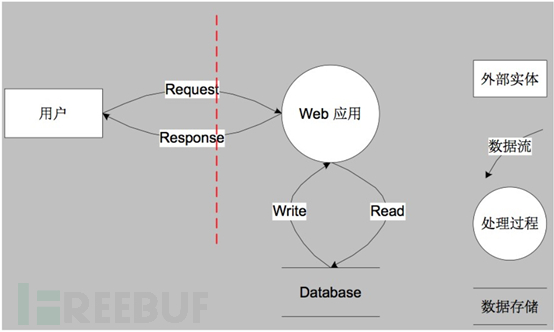
\includegraphics[scale=0.6]{resources/img/i5.png}
%     \caption{简单数据流图实例}
%   \end{figure}


\subsubsection{STRIDE四类元素与六类威胁的对应关系}

具体的对应关系如图2.5示例,并不是每个元素都会面临6个威胁,比如外部实体只有仿冒和抵赖两类威胁,我们不用关心外部实体会不会被篡改、会不会发生信息泄露、以及拒绝服务等,因为外部实体本来就是我们控制范围之外的。

其中进程(处理过程)会面临全部的6个威胁,数据存储中Repudiation(抵赖)是红色,表示只有存储的数据是审计类日志才会有抵赖的风险,存储其他数据的时候无抵赖。
\begin{figure}
    \centering
    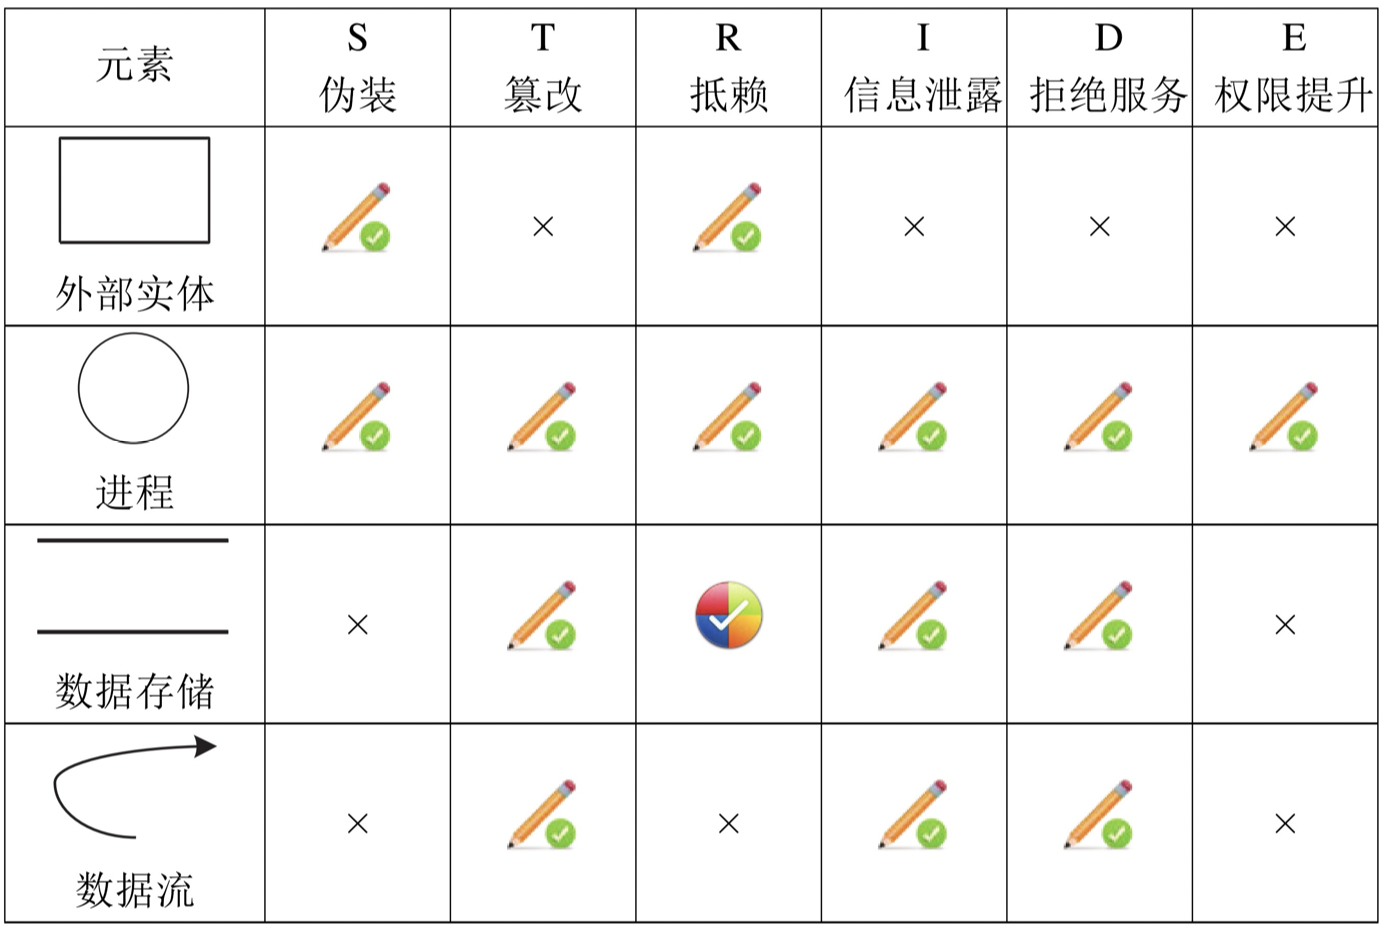
\includegraphics[scale=0.6]{resources/img/i77.png}
    \caption{四类元素和六类威胁对应关系}
  \end{figure}

\subsubsection{STRIDE 威胁建模流程}
(1) 分解业务场景,画出数据流关系图(DFD)威胁建模针对的是具体场景,
所以应该根据实际应用场景对业务进行分类,比如购买场景和注册场景等。至于有
多少个场景或怎么分类是根据用户使用的系统以及业务息息相关。比如淘宝、京东
与拼多多等电商系统,国外 Amazon EC2 和国内的腾讯云系统。这些系统分解出的业务场景肯定是不相同的。每种业务每种场景对应的
STRIDE 威胁建模是独立、互不干扰的,因此需要对分解完业务场景的每一个场景进
行单独的 STRIDE 威胁建模。接着就需要绘制数据流关系图。数据流关系图由数据
流(箭头)、数据存储(双横线)、进程(圆形)和外部实体/交互方(方形)四个元
素标准符号组成。如图 2.6 所示。
除了上述四种核心组件外,根据实际情况,可能还需要增加一个元素,称为信
任边界,在途中我们用虚线表示。当数据流在不同的信任边界上流动,就需要用虚
线来区分不同的信任区域。由于信任边界在后续的建模威胁分析种,多数不会被分
析,因此,核心元素大多只包含:进程、数据存储、数据流和交互方/外部实体四钟,
并不包含所谓的信任边界。添加信任边界后,需要对每一个节点每一段数据流进行
分析,判断是否存在 6 个维度的安全威胁。

\begin{figure}
    \centering
    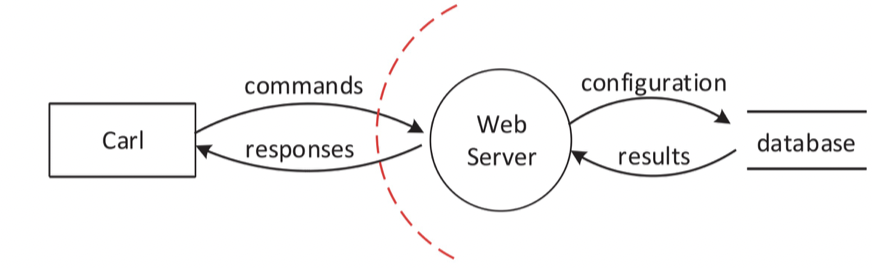
\includegraphics[scale=0.6]{resources/img/i7.png}
    \caption{常用web场景数据流图}
  \end{figure}
  (2)列出节点元素的安全威胁,逐个具体分析。绘制完数据流图之后,需要列
  出数据流中的每个节点元素可能面临的安全威胁,并逐个分析,当然也不是需要对
  每个元素的 STRIDE 威胁都要进行分析。如表 2.1 所示。
  表中列出了每种元素可能面临的安全威胁,从中能够看出只有进程才有可能面
  临 STRIDE 所有威胁,即需要对六种威胁逐个分析。外部实体可能面临“伪装”和
  “抵赖”两种威胁,数据流需要分析“篡改(替换)”、“信息丢失或泄露”和“拒绝
  服务”三种威胁。需要注意的是 R 选项勾选的是不一样的颜色,对于数据存储这个
  元素,意思是“抵赖”这个威胁可能有,也有可能没有,当数据用作审计的时候,需
  要分析“抵赖”威胁,其他情况不需要考虑这个威胁。
  \begin{table}
    \caption{元素STRIDE威胁分析}
  \begin{center}
    \begin{tabular}{|l|l|l|l|l|l|l}
      \hline 元素类型 & 伪装 & 篡改 & 抵赖 & 信息泄露 & 拒绝服务 & 权限提升\\
      \hline 外部实体 & X & X & X & X & X & X \\
      \hline 进程 & X & X & X & X & X & X \\
      \hline 数据存储 & X & X & X & X & X & X \\
      \hline 数据流 & X & X & X & X & X & X \\
      \hline
      \end{tabular}
  \end{center}
\end{table}
  (3)输出威胁列表包括消减方案和威胁评级。分析完数据流图中所有元素即所
有对象的潜在安全威胁之后,需要输出一个威胁列表。如表2.2 就是一个典型的威胁
列表。威胁列表本身不能说是一个方法论,只能说是相关工作的结果,是威胁建模
中一个辅助的列表,能够帮助我们进一步分析威胁,进一步提高威胁建模的准确度。
其中,消减方案和危险评级是需要重点分析的两项。
\begin{table}
  \caption{威胁列表}
\begin{center}
  \begin{tabular}{|l|l|}
    \hline 组件(威胁的目标) & App 应用程序用户身份验证进程 \\
    \hline 威胁描述 & 攻击者通过中间人攻击获取身份验证凭据 \\
    \hline 威胁类别 & I \\
    \hline 攻击方法 & 利用网络监视软件 \\
    \hline 消减方案(对策) & 利用 SSL/TLS 提供加密通道 \\
    \hline 危险评级 & 待定 \\
    \hline
    \end{tabular}
\end{center}
\end{table}
危险评级,根据造成的影响对威胁进行评价打分。这样可以将威胁进行分类,
首先解决威胁最大的安全风险,再解决其他的安全威胁。威胁的评级方法繁多,以
安全漏洞评级为例,主要有 DREAD 和 CVSS(Common Vulnerability Scoring System,
通用漏洞评估方法)两种评级方法。不同的评级方法考虑的维度和计算方法略有差
异,但本质上来说,威胁级别 = 威胁发生的概率 × 威胁带来的损失,这个公式是没
有变化的。具体用哪种危险评级方法,因根据实际情况来决定。

DREAD 名称类似于 STRIDE,是威胁评级 6 个指标的英文首字母,即 Damage
Potential(潜在损失)指漏洞被利用会造成的经济损失;Reproducibility(重现性)指
再次攻击的难度;Exploitability(可利用性)指攻击的难难程度;Affected users(影
响的用户)用粗略的百分数表示有多少用户受到影响;Discoverability(被发现性)
指发现的难易程度。最终的威胁评级由这 6 个指标加权平均计算得出,公式如下
$$
\operatorname{Rank}[0: 10]=\frac{(D a m+\operatorname{Rep}+\operatorname{Exp}+A f f+\text { Dis })}{2}
$$


Rank 表示威胁评分,范围从 0 到 10,表示从无危险到极度危险。这个公式并不是统
一的标准,之所以采用这样的计算方式,是为了让威胁等级的分数范围与 CVSS 范
围相同。每项指标的分数从 0 到 4,表示严重程度逐渐增加,如表 2.5 所示,没有列
出等级 0,是因为 0 表示没有这个威胁。
\begin{table}
  \caption{威胁评级}
\begin{center}
  \begin{tabular}{|l|l|l|l|l|}
    \hline 等级 & 极高(4) & 高(3) & 中(2) & 低(1) \\
    \hline 潜在的损失D & 获取最高权限 & 泄露关键信息 & 泄露敏感信息 & 泄露其他信息 \\
    \hline 重现性R & 可随时攻击 & 易重复攻击 & 可重复攻击 & 难重复攻击 \\
    \hline 可利用性E & 非常容易利用 & 较为容易攻击 & 高级黑客可利用 & 攻击条件苛刻 \\
    \hline 受影响用户A & 所有用户 & 管理员 & 一般用户 & 其他用户 \\
    \hline 可发现性D & 漏洞过于明显 & 需要漏洞挖掘 & 限定范围可发现 & 隐藏性极高 \\
    \hline
    \end{tabular}
\end{center}
\end{table}

\subsection{攻击树模型}

攻击树模型是 Schneier\cite{schneier1999attack} 提出的一种系统攻击
分类方法。这种方法采用树形结构描述攻击逻辑,使
安全分析人员从系统面临攻击威胁的角度思考安全问
题。利用树形结构的优势,可以用简单的结构描述复
杂的威胁类型和攻击方式,具有很强的扩展性 \cite{tuozhan}
,便
于从深度、广度不同的层次对攻击逻辑做出修正,从
而帮助分析者构建系统、全面的安全威胁模型
一个完整的树形结构包括根节点、分支节点和
叶子节点。在攻击树中,根节点表示最终要实现的
攻击目标,分支节点表示要完成最终目标所要完成
的中间步骤,叶子节点表示具体的攻击方法。兄弟
节点间可以反映一定的攻击逻辑,如图2.7所示。“或
(OR)”关系表示任意子节点的方法得到实现,
其父节点的攻击目标才会实现;“与(AND)”关系表示只有当所有子节点目标都得到实现,父节点
的攻击目标才会实现;“顺序(SAND)”关系表
示所有子节点目标按照顺序实现后,父节点的攻击
目标才会被实现。攻击树的每一条路径都表示一种
攻击方案所要遵循的基本路线,路径的深度也间接
反映该攻击方法的难易程度。
一旦树建立起来,就可以为各个叶节点分配值,然后使关于节点的计算。一旦分配了值,就可以计算安全性的目标。
攻击属性有助于将风险与攻击联系起来。
攻击树可以看作一个包括所需的特殊知识或设备,完成所需的时间完成一个步骤,以及攻击者衡量承担的物理和法律风险。
攻击树中的每个节点值也可能是运营或开发费用。攻击树支持设计和需求决策。如果攻击成本多于利益,
即攻击很可能不会发生。但是,如果攻击者发现有可得利益则会攻击 因此需要防御。

\begin{figure}
    \centering
    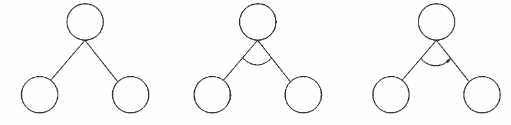
\includegraphics[scale=0.6]{resources/img/i8.png}
    \caption{攻击树基本结构}
  \end{figure}

\subsection{CVSS模型}

通用漏洞评分系统(CVSS)(2007 年完成,第 2 版)被认为是衡量软件漏洞相对严重性的规范,可应用于大
量系统,包括那些属于美国联邦机构的系统\cite{mell2007common}。
CVSS 由三个不同的度量组组成:基础、时间和环境。每一个都由它们自己的一套度量标
准组成。基本度量组可用于大多数情况,但也可以将其他值分配给其他度量组,以便为特定漏洞提供额
外的上下文。这些度量组可以描述如下:
\begin{itemize}
    \item  基础表示漏洞的特征,这些特征会随着时间和用户环境的变化而不断变化
    \item  时态表示漏洞随时间变化的特征,但不提及用户环境
    \item  环境表示与用户的特定环境相关和/或独特的漏洞特征
\end{itemize}

一旦为这些基本指标中的每一个分配了一个值,基本公式就会计算出一个范围从 0 到 10 的分数。根据所
有因素,从等式中创建一个向量,并将该向量输出为包含分配给每个指标的值的文本字符串,以便准确
传达如何为每个发现的漏洞得出分数。该过程如图 2.8 所示。
\begin{figure}
    \centering
    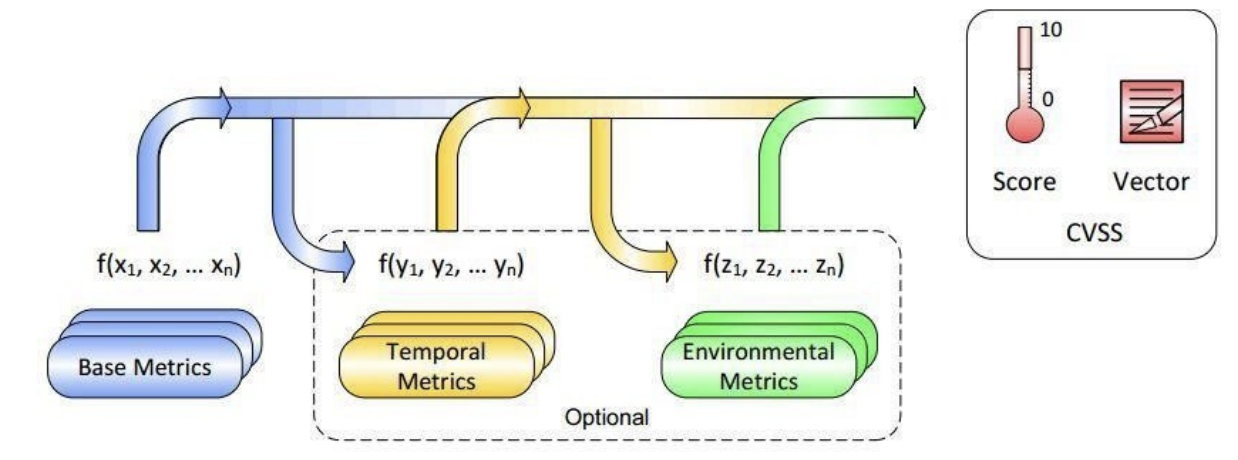
\includegraphics[scale=0.6]{resources/img/i9.png}
    \caption{CVSS的度量和方程组合起来创建矢量}
  \end{figure}

  \subsection{HEAVENS安全模型}
  如图2.9所示,HEAVENS安全模型\cite{haringajoint}旨在识别所有者、资产、风险、漏洞、对策、威胁代理和威胁,并将所有方面
整合在一起,以建立汽车行业的安全模型。此外,我们的目标是在汽车电子/电子系统的背景下研究来
自其他领域(例如,IT 安全、电信和国防)的安全模型。因此,在HEAVENS安全模型中,第一步是从涉众(即
所有者)的角度识别用例。用例随后被用于识别资产和威
胁,包括可能受到特定威胁影响的安全属性。在风险评估期间,威胁代理(攻击者)的角色以及攻击对特
定资产的影响已被考虑,以对威胁进行评级,即识别风险。这有助于确定安全要求和可能的对策,以解
决特定资产的特定威胁。

\begin{figure}
    \centering
    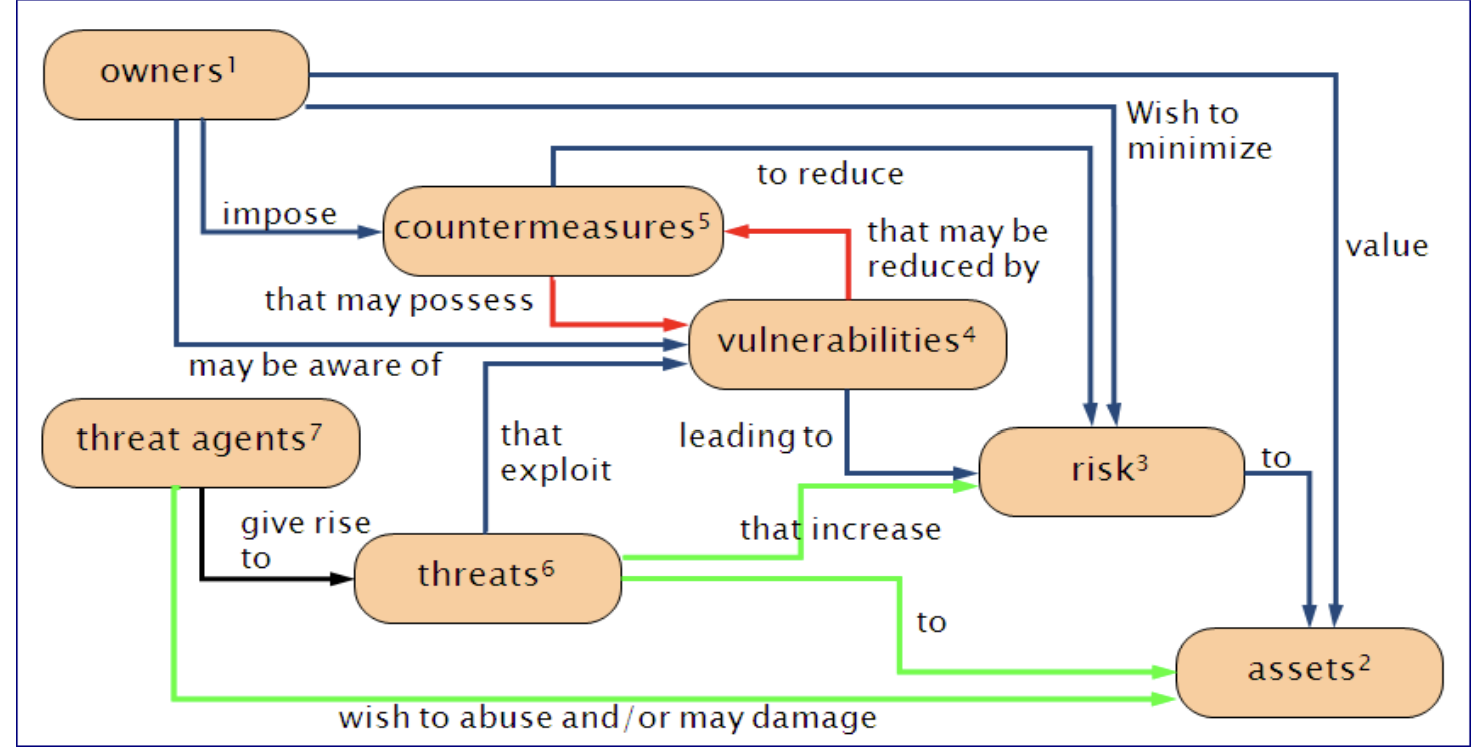
\includegraphics[scale=0.6]{resources/img/i10.png}
    \caption{典型的威胁风险评估图}
  \end{figure}

  HEAVENS安全模式的优势如下:

  \begin{itemize}
    \item  所提出的模型同样适用于各种道路车辆,例如客车和商用车。该模型考虑了广泛的利益相关方 (例
    如,原始设备制造商、车队所有者、车主、驾驶员、乘客等)。
    \item  时通过在汽车电子电气系统环境中应用微软的 STRIDE 方法实现的以威胁为中心的模型。它通过仅使用
    少数通用威胁类别,而不是考虑与资产相关的几乎无限的攻击可能性和攻击技术,来支持更好地理
    解可能的攻击的影响。
    \item  该模型在威胁分析期间建立了安全属性和威胁之间的直接映射。这有助于对特定资产的特定威胁的
    技术影响(机密性、完整性、可用性)进行可视化和早期评估。
    \item 该模型将安全目标(安全、财务、运营、隐私和法规)与风险评估期间的影响级别估计对应起来。这
    有助于了解特定威胁对相关利益方(例如 OEM)的潜在业务影响。
    \item 该模型符合成熟的行业标准和计划。例如,通用标准ISO-26262。这有助于
    重用其他研究领域已经存在的过程,例如,功能安全。它还提供了一个了解跨安全和安保领域的网
    络安全问题的机会。
\end{itemize}

HEAVENS安全模型的主要目标是推导出TOE的安全要求,即TOE的资产,类似于ISO-26262中所述的功能安全要求的概念。
为了实现这一点,我们为与构成 TOE 的资产相关的每个已识别的
威胁建立了一个安全级别。因此,HEAVENS安全模型包括威胁分析和风险评估。因此,“HEAVENS安全模型”指
的是威胁分析和风险评估,以便通过应用HEAVENS方法和工具支持来推导特定 TOE 的安全要求。
图 2.10 显示了HEAVENS安全模型的工作流程。它由三部分组成——威胁分析、风险评估和安全要求。
HEAVENS安全模型的工作流程如下:
\begin{itemize}
    \item  威胁分析–功能用例的描述(图中的 In\_01)是威胁分析流程的输入。威胁分析产生两个输出:(a)用例环境中每个资产的威胁和资产之间的映射(图中的Out\_01),
    以及(b)威胁和安全属性之间的映射(图中的Out\_02),以确定哪些安全属性由于资产环境中的特定威胁而受到影响。
    \item  风险评估—一旦确定了相关资产的威胁,下一步就是对威胁进行分级。这是在风险评估期间完成的。威胁和资产之间的映射与威胁级别(TL)(图中的 In\_03)和影响级别(IL)
    (图中的 In\_04)参数一起用作输入。作为风险评估的最终结果,我们为与TOE/用例的每个资产相关联的每个威胁确定安全级别(图中的 Out\_03)。
    \item  安全要求–最后,我们考虑威胁和资产之间的映射(图中的 Out\_02 是威胁分析的结果)以及安全级别(图中的 Out\_03 是风险评估的结果)来制定资产和 TOE 的安全要求。
    安全需求是资产、威胁、安全级别和安全属性的函数。请注意,安全级别根据与特定资产相关联的特定威胁的安全目标来考虑潜在的业务影响。
    衍生的安全要求处于 ISO-26262 功能安全要求的水平,属于概念阶段。之后,在产品开发阶段,需要根据高级安全需求派生出软件安全需求和硬件安全需求。
  \end{itemize}


\begin{figure}
    \centering
    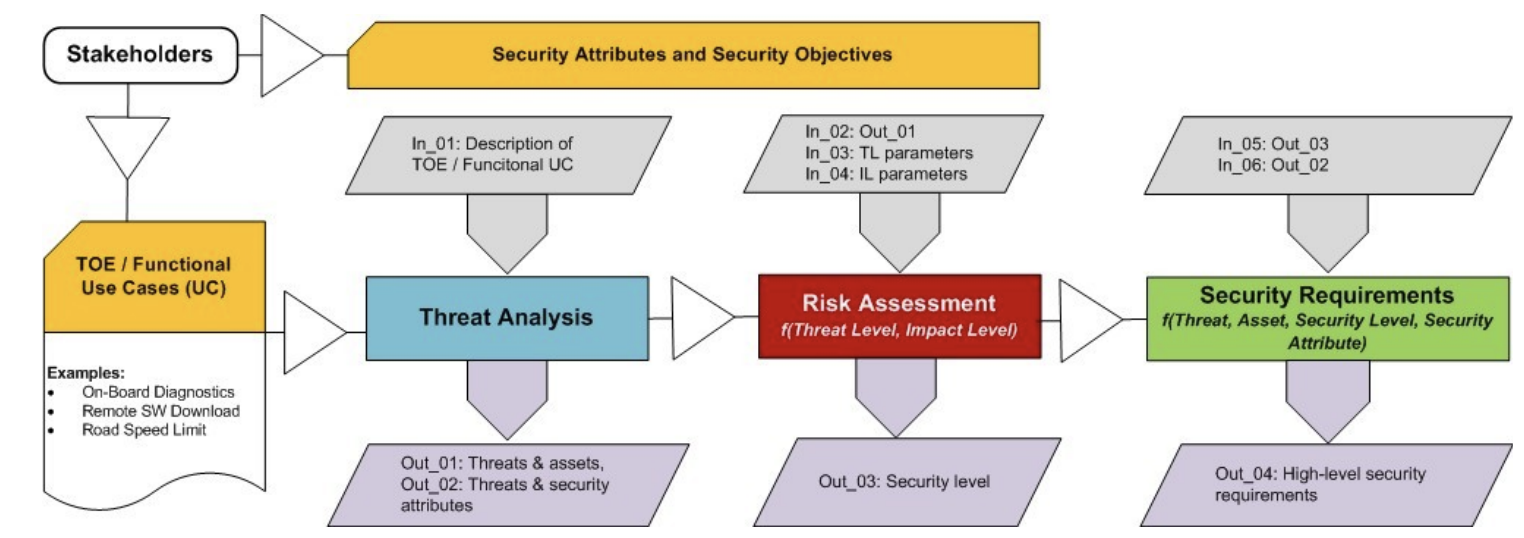
\includegraphics[scale=0.6]{resources/img/i11.png}
    \caption{HEAVENS安全模型工作流程图}
  \end{figure}

  \section{层次分析法和FAHP}
  这里我们介绍下层次分析法用于第四章进行新的安全模型的理论基础。
  AHP 是一种结合定性和定量分析的多目标决策分析方
法,由萨蒂在20世纪70年代提出\cite{saaty1990make}。这种方法的主
要思想是通过将复杂的问题分解成几个层次来比较每两
个决策元素的相对重要性,每个层次由有限数量的决策
元素组成。然后建立满足性质(2)(3)的判断矩阵。通过
计算判断矩阵的最大特征值和相应的特征向量,从两两
比较中间接评估不同元素的相对重要性。层次分析法的
特点是将人们的主观判断数学化,使决策更容易被接
受。AHP 的过程可分为以下步骤:
\begin{itemize}
  \item  构建一个问题的层次结构,包括一个目标、实现
  目标的要素以及对这些要素进行评分的评估标
  准。
  \item  将决策元素成对比较,根据标度准则确定相对
  重要性,然后构造一个判断。
  \item  计算每个元素的权重并检查判断矩阵的一致
  性。
  \item 通过比较综合重要性,根据所有备选方案的优先
  级做出最终决策。
\end{itemize}

然而,层次分析法难以检查判断矩阵的一致性,其一
致性判断准则缺乏科学依据。此外,当有许多评价指标
时,很难保证决策的一致性。在这种情况下,FAHP 应运而
生\cite{min1997fuzzy}。一种是基于模糊数的 FAHP,另一种是基于模糊判
断矩阵的。FAHP 的过程与层次分析法相同,但仍有两个
不同之处:
\begin{itemize}
  \item  建立的判断矩阵不同:层次分析法是判断矩阵,而
  FAHP 是模糊判断矩阵
  判断矩阵。
  \item  寻找矩阵中每个元素相对重要性的不同加权方
  法。
\end{itemize}


\section{本章小结}

本章主要介绍了智能网联汽车的系统架构,首先从整体上给出其车联网系
统的架构介绍,然后对 TSP 云服务、V2X,车载网络通信进行了详细分
析,解释了车载网络通信各个协议之前的区别和优劣。
然后介绍了三种类型的威胁方面。最后主要介绍智能网联汽车领域的威胁建模分析:
首先介绍传统的 STRIDE 模型,攻击树模型,CVSS 和 新型的HEAVES安全模型.此外还介绍了AHP和FAHP层次分析法用于定量分析。
为后文叙述系统架构中存在的攻击入口以及漏洞打下基础。
为后续的智能互联汽车威胁模型的提出提供了前置理论来源。